\section{Models and Results}
\label{sec:Models and Results}
This section presents a summary of each model's performance and includes key visualizations to illustrate their predictive capabilities.
A decision threshold of 0.5 was used for all models producing continuous predictions — i.e., predictions were classified as class 1 if the output 
was greater than 0.5, and as class 0 otherwise.

\subsection{Baselines: Random and Majority Guessing}

As a baseline, we implemented two trivial classifiers:

\begin{itemize}
    \item \textbf{Random Guessing}: Each image was randomly labeled as either \texttt{CIFAR-10} or \texttt{ImageNet} with 50\% probability. Over 100 runs, this yielded a mean accuracy of approximately \textbf{50\%}.
    \item \textbf{Majority Guessing}: Always predicting the dominant class (\texttt{ImageNet}) led to a test accuracy of \textbf{78\%}.
\end{itemize}

These baselines confirm that a high accuracy can be misleading in imbalanced datasets, emphasizing the need for more informative metrics.

\subsection{Random Forest Classifier}

Our non-deep learning benchmark was built using scikit-learn's \texttt{RandomForestClassifier}. We tested all combinations of the parameters 
\texttt{n\_estimators} (100, 150), \texttt{max\_depth} (None, 10, 20), \texttt{min\_samples\_split} (2, 5, 10), \texttt{max\_features} (\texttt{sqrt}, \texttt{log2}), 
and \texttt{criterion} (\texttt{gini}, \texttt{entropy}, \texttt{log\_loss}). The best performing model achieved an accuracy of \textbf{78.53\%}, 
which is again close to majority guessing. It predicted \texttt{ImageNet} in 89,188 out of 90,000 cases, thus strongly favouring the \texttt{ImageNet} domain.

%Our non-deep learning benchmark, was build using scikit-learn's \texttt{RandomForestClassifier}.
%Using the parameter candidates
%\begin{itemize}
%    \item \texttt{n\_estimators}: 100, 150
%    \item \texttt{max\_depth}: None, 10, 20
%    \item \texttt{min\_samples\_split}: 2, 5, 10
%    \item \texttt{max\_features}: \texttt{sqrt}, \texttt{log2}
%    \item \texttt{criterion}: \texttt{gini}, \texttt{entropy}, \texttt{log\_loss}
%\end{itemize}
%we created all possible parameter combinations.
%The best performing model achieved an accuracy of \textbf{78.53\%}, again close to majority guessing.
%It predicted \texttt{ImageNet} in 89,188 out of 90,000 cases thus strongly favouring \texttt{ImageNet}.

\subsection{Fully Connected Neural Network (MLP)}
The used MLP model used the architecture
\begin{itemize}
    \item Flatten → Dense(512, ReLU) → BatchNorm → Dropout(0.3)
    \item Dense(256, ReLU) → BatchNorm → Dropout(0.3)
    \item Dense(1, Sigmoid)
\end{itemize}
and reached a test accuracy of \textbf{78\%}, predicting \texttt{ImageNet} for 88,828 out of 90,000 test images. 
This again aligns with the majority baseline, showing that without spatial features, the model mostly learns the class imbalance.

\subsection{Minimal CNN for Visualization}
For interpretability, we trained a minimal convolutional network designed to extract and visualize learned kernels and feature maps:
\begin{itemize}
    \item Conv2D(2 filters)(3x3 Kernel) → MaxPooling2D → Flatten → Dense(1, Sigmoid)
\end{itemize}
Despite its simplicity, this model achieved a \textbf{96\%} test accuracy, with F1-scores of \textbf{0.91} for \texttt{CIFAR-10} and \textbf{0.97} for \texttt{ImageNet}. 
However, due to its limited use in drawing insights, we include its kernel and filtered image visualizations only in the 
Appendix~\ref{sec:Filter and Activation Visualizations — Minimal CNN}.

\newpage
\subsection{CNN with Hyperparameter Optimization}
We then developed a moderately complex (compared to the model before) CNN and optimized its hyperparameters using the optimization framework \texttt{Keras Tuner}~\cite{omalley2019kerastuner}. 

\setlength\intextsep{0pt}
\begin{wrapfigure}[12]{r}{0.5\textwidth}
    \begin{center}
        \vspace{-\baselineskip}
        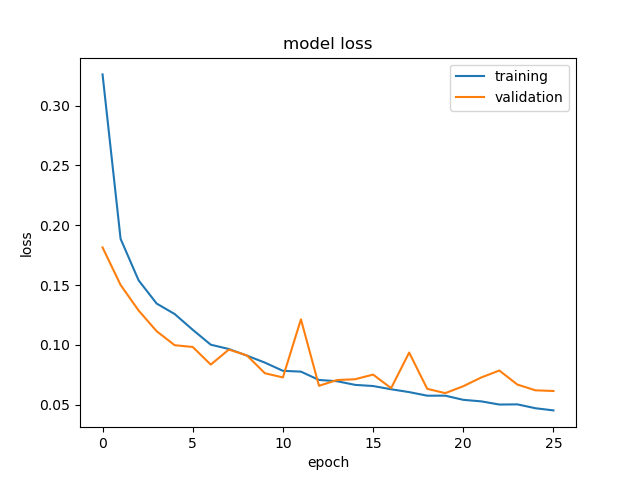
\includegraphics[width =0.48\textwidth]{Plots/ModelsAndResults/Hyperparameter_search_Loss.png}
        \caption{Training and validation loss of the CNN with Parameter ID P00.}
        \label{fig:hyperparameter_loss_plot}
    \end{center}
\end{wrapfigure}

The search space included Conv layer filter count and kernel size, use of a second Conv layer, Dropout rate, Dense layer units and the Learning rate.

Out of many configurations, the best CNN achieved the following on the test set
\begin{itemize}
    \item \textbf{Accuracy}: 98.19\%
    \item \textbf{F1-score (CIFAR-10)}: 0.96
    \item \textbf{F1-score (ImageNet)}: 0.99
\end{itemize}
and the training performance on the training and validation set over multiple epochs is shown in \autoref{fig:hyperparameter_loss_plot}.

To better understand how different hyperparameter configurations influenced the validation accuracy of our CNN model, 
\autoref{fig:Hyperparameter_Config_plot} visualizes the validation accuracy across tested configurations.
A sample of the configuration details is listed in \autoref{tab:Hyperparameter_Config_tab} in Appendix~\ref{sec:Hyperparameter Configurations}.

\begin{figure}[H]
    \centering
    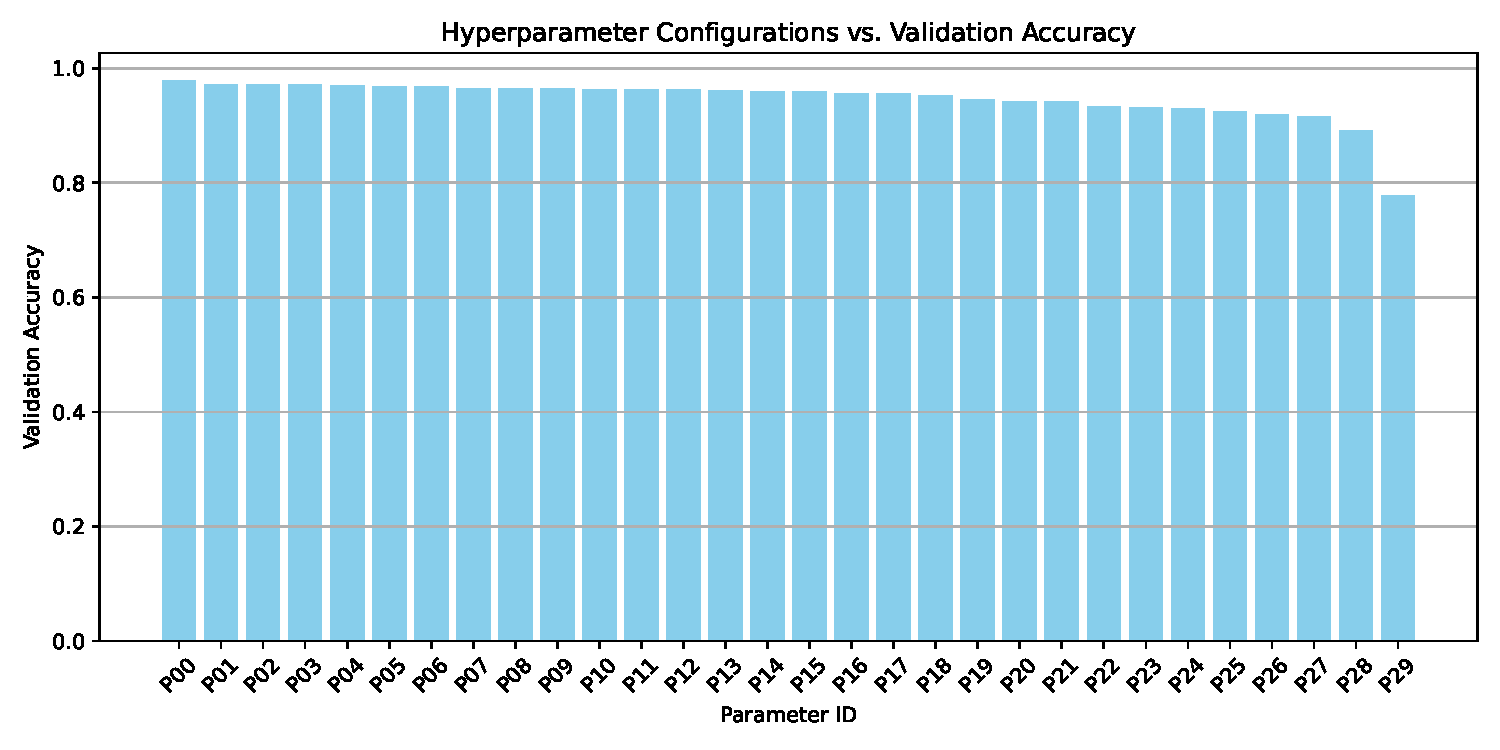
\includegraphics[width=0.9\textwidth]{Plots/ModelsAndResults/Hyperparameter_Config_plot.pdf}
    \caption{Validation accuracy for selected hyperparameter configurations tested with Keras Tuner. Each configuration ID corresponds to one model setup.}
    \label{fig:Hyperparameter_Config_plot}
\end{figure}

\raggedbottom
\addtolength{\topskip}{0pt plus 10pt}
This model demonstrated that with enough capacity and tuning, even modest CNNs can learn highly predictive domain-specific features.


\subsection{ResNet-18}

To evaluate how well a deeper architecture performs, we trained a \textbf{ResNet-18} model~\cite{he2016ResNet18} on the same binary classification task. 
Without any hyperparameter tuning, the model reached:

\begin{itemize}
    \item \textbf{Accuracy}: 99.26\%
    \item \textbf{F1-score (CIFAR-10)}: 0.98
    \item \textbf{F1-score (ImageNet)}: 1.00
\end{itemize}

\autoref{fig:ResNet18_loss_plot} illustrates the loss and validation performance over the training epochs, suggesting the models capabilities being bigger then needed.  
To further analyze performance, we include \autoref{fig:ResNet18_confusion_matrix_plot}, which presents the confusion matrix for test predictions. 
The nearly perfect separation between CIFAR-10 and ImageNet images supports the conclusion that this deep model can exploit source-specific characteristics with high reliability.

\begin{figure}[H]
    \centering
    \begin{subfigure}[b]{0.48\textwidth}
        \centering
        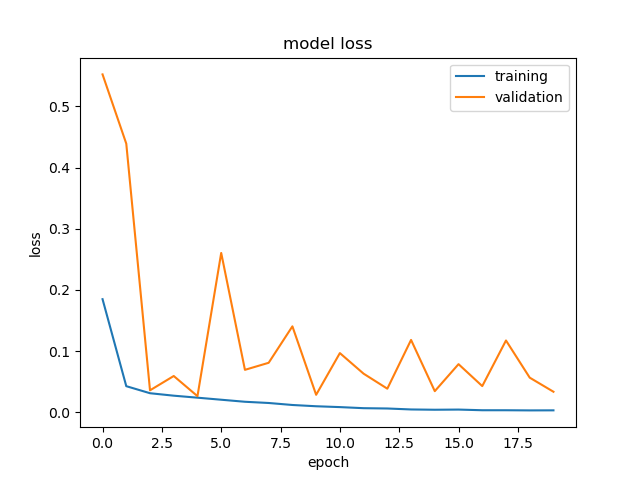
\includegraphics[width=\textwidth]{Plots/ModelsAndResults/ResNet18_Loss.png}
        \caption{Loss and validation accuracy of ResNet-18 during training.}
        \label{fig:ResNet18_loss_plot}
    \end{subfigure}
    \hfill
    \begin{subfigure}[b]{0.48\textwidth}
        \centering
        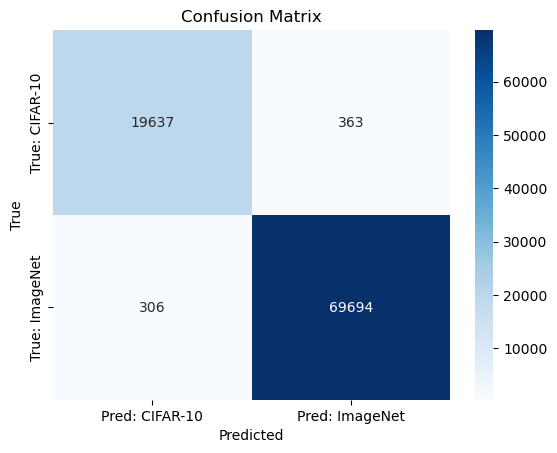
\includegraphics[width=\textwidth]{Plots/ModelsAndResults/ResNet18_confusion_matrix.png}
        \caption{Confusion matrix of ResNet-18 predictions on the test data.}
        \label{fig:ResNet18_confusion_matrix_plot}
    \end{subfigure}
    \caption{Training behavior and evaluation of ResNet-18 model.}
    \label{fig:ResNet18_combined}
\end{figure}

These results confirm that deep architectures like ResNet-18 can achieve near-perfect source discrimination, setting a strong upper performance bound for this task.